\chapter{Our contributions}
\label{kap:kap3}

In this chapter, we propose various ideas that we hope lead to a better practical
implementation of RRR. We first propose a new general block encoding and decoding routine.
Then, we show how we can exploit the assumptions about the represented bit sequence to
come up with implementation that is better tailored for the concrete bit sequence in terms of
the query time and space usage.

\section{Block encoding}

As we discussed in section~\ref{section:compressed_bv}, there are to
the best of our knowledge two widely used methods to encode and decode the
blocks in RRR. Disadvantage of the table decoding method is its inability
to reasonably support longer blocks in practice because of the huge size of
helper tables. On the other hand, the on-the-fly decoding method may be used
to support a longer blocks with the downside being longer encoding and decoding
times. In this section, we propose a new method for block encoding and decoding.
The main objective of the new method is to enable use of longer blocks while not
hurting the runtime so significantly.

The main idea of our proposed solution is to use a divide-and-conquer approach to
break the problem of finding the order of the block $B$ along the class $c$ to
the finding of order of several smaller sub-blocks of $B$. The potential advantage of this
solution is that it may enable us to use the table method to solve the smaller
subproblems. To facilitate our solution, we altered the respective order of the blocks
along the class and we do not use the lexicographical ordering anymore. Note that we
continue to use the number of ones to identify class of the block. In our solution, every
block $B$ will be thought of as a concatenation of two smaller \textit{sub-blocks}, $B_1$
and $B_2$. Primarily, the blocks are ordered according to the value of their \textit{class pair}
$(c_1, c_2)$ where $c_1$ and $c_2$ are the classes of the smaller sub-blocks $B_1$ and $B_2$,
respectively. Only then, the tie is broken by order of $B_1$ and $B_2$ along their respective
classes. An example of the new ordering for blocks of length 6 is shown in Fig.~\ref{obr:lexicographicalVsUs}.

\begin{figure}
	\centerline{
        \begin{tabular}{l c l}
            Offset  &   Block       & $(c_1, c_2)$\\
        \hline
            \small 0&   \tt 000 011 & \multirow{3}{*}{$(0, 2)$}\\
            \small 1&   \tt 000 101 & \\
            \small 2&   \tt 000 110 & \\
        \hline
            \small 3&   \tt 001 001 & \multirow{5}{*}{$(1, 1)$}\\
            \small 4&   \tt 001 010 &\\
            \small 5&   \tt 001 100 &\\
            \small 6&   \tt 010 001 &\\
            \small 7&   \tt 010 010 &\\
        \end{tabular}
        \hspace{3em}
        \begin{tabular}{l c l}
            Offset  &   Block       & $(c_1, c_2)$\\
        \hline
            \small 8&   \tt 010 100 & \multirow{4}{*}{$(1, 1)$}\\
            \small 9&   \tt 100 001 &\\
            \small 10&  \tt 100 010 &\\
            \small 11&  \tt 100 100 & \\
        \hline
            \small 12&  \tt 011 000 & \multirow{3}{*}{$(2, 0)$}\\
            \small 13&  \tt 101 000 &\\
            \small 14&  \tt 110 000 &\\
        \end{tabular}
	}
	\caption[TODO]{
        The example of new ordering for the block length $b=6$ and class $c=2$.
        Every block is divided into two sub-blocks of length 3. Note the differences to the
        lexicographical ordering. Block {\tt 011 000} on offset 12 is preceded by lexicographicaly
        greater blocks {\tt 100 001}, {\tt 100 010} and {\tt 100 100} as it has bigger number of ones
        in the first sub-block.
    }
	\label{obr:lexicographicalVsUs}
\end{figure}

Formalizing this, we shall write $B\prec_X B'$ if blocks $B$ and $B'$ are of
the same length, class and at the same time $B$ precedes $B'$ in ordering $X$.
In this situation, we often refer to block $B$ as being smaller than $B'$.
We write $B\prec_{\Lex} B'$ if $B$ precedes $B'$ in lexicographical ordering.
Using this new notation, our new proposed ordering $P$ can be formalized as:
\begin{align*}
    B\prec_P B' \iff
    &[\#_1(B_1) < \#_1(B_1')] \\
    &\lor [(\#_1(B_1) = \#_1(B_1')) \land B_1 \prec_{X} B_1']\\
    &\lor [B_1 = B_1' \land B_2 \prec_{Y} B_2']
\end{align*}
where $B=B_1\cdot B_2$, $B'=B_1'\cdot B_2'$ and $X$, $Y$ are arbitrary orderings.
Note that both $X$ and $Y$ do not have to be lexicographical orderings but can also again
use our new ordering $P$.

In the rest of this section, we are going to explain how encoding and decoding works
with our proposed ordering.

\paragraph{Encoding}

Before providing the general encoding routine, let us demonstrate the process on
a simple example and then generalize the ideas behind the process. Imagine
encoding block {\tt 100010} of length 6. Let us encode this block using our new
subroutine with 3 as a sub-block length. We may observe that the class of this
block is 2 as there are two ones in the whole block. Obtaining the offset is
more complicated. We calculate it by enumerating the number of blocks preceding
{\tt 100 010} in the class $c=2$. We divide the blocks preceding {\tt 100 010}
into 3 categories:
\begin{itemize}
    \item Blocks with a smaller number of ones in the first sub-block.
    (There are 3 such blocks -- those beginning with {\tt 000}.)
    \item Blocks with the same number of ones in the first sub-block, but smaller first sub-block.
    (There are 6 blocks with this property -- those beginning with {\tt 010} or {\tt 001}.)
    \item Blocks with the same first sub-block, but smaller second sub-block.
    (There is 1 such block, namely {\tt 100 001}.)
\end{itemize}
Summing up, we get that there are 10 blocks preceding {\tt 100 010} so it follows
that its offset $o$ is equal to 10 (when indexing from 0). Together with its class,
we encode this block as a pair of numbers $(2, 10)$.

Let us generalize the process of encoding block $B$ of length $b$
with sub-blocks of length $b_1$ and $b_2$. We also need two orderings $X$ and $Y$
that can be used to order sub-blocks $B_1$ and $B_2$, respectively.
The first step is to count the number of ones to obtain class $c=\#_1(B)$.
Then we compute the offset by counting the number of blocks $B'$ preceding $B$.
These can be divided into 3 categories:
\begin{enumerate}
    \item $B'$ such that $\#_1(B'_1) < \#_1(B_1)$
    \label{chapter3:encoding:1}
    \item $B'$ such that $\#_1(B'_1) = \#_1(B_1), B'_1\prec_X B_1$
    \label{chapter3:encoding:2}
    \item $B'$ such that $B'_1 = B_1, B'_2\prec_Y B_2$
    \label{chapter3:encoding:3}
\end{enumerate}
One can observe that these categories closely resemble the definition of our ordering
in the previous paragraph.

The number of blocks in the first category~\ref{chapter3:encoding:1} is equal to
$$\sum_{i=0}^{c_1-1} {b_1\choose i} {b_2\choose c-i}.$$ For fixed $i$, ${b_1\choose i}$
denotes the number of sub-blocks with $i$ ones and ${b_2\choose c-i}$ denotes the number
of sub-blocks with the rest $c-i$ ones.

The number of blocks in the second category~\ref{chapter3:encoding:2} is equal to
$$o_1\times {b_2\choose c_2}.$$ These are all the blocks with first sub-block smaller
than $B_1$ and any second sub-block with $c_2$ ones.

The number of blocks in the third category~\ref{chapter3:encoding:3} is equal to $o_2$.
This is number of blocks that have $B_1$ as the first sub-block and smaller second
sub-block $B_2$.

As we mentioned, the offset of block $B$ is given by the sum of sizes of these 3 groups.
However, to obtain these, we need to get $c_1, c_2, o_1$ and $o_2$. These numbers can be
obtained by recursively encoding the sub-blocks $B_1$ and $B_2$.

\paragraph{Decoding}

Decoding is a process of obtaining bit representation of block $B$ from its encoded
representation $(c, o)$. When our new encoding scheme is used, main part
of the decoding process is to obtain encoded representations $(c_1, o_1)$ and
$(c_2, o_2)$ of sub-blocks $B_1$ and $B_2$. These two can then be fed into
the decoding subroutines to obtain sub-blocks $B_1$ and $B_2$. Concatenating these
two representations gives us the decoded block $B$.

% TODO: mozno ked bude cas sa k tomu mozme vratit ale bud to chce zmenit cisla
% na ktorych ten priklad robim alebo neviem, nedava mi ziadnu value ten priklad

%We shall again present this process on an example and decode the block $B$ from the previous
%encoding example {\tt 100 010} encoded as $(2, 10)$.

%The first step is to obtain the class pair of block $B$. This is pair of classes
%of sub-block. We can use the table in Fig.~\ref{obr:lexicographicalVsUs} and see
%that there are 3 blocks with class pair $(0, 2)$. As the offset of our block is 10,
%we need to look for this block between blocks with bigger class pair. There are 9
%blocks with class pair $(1, 1)$. As $3+9$ is bigger than 10, we can say that the
%class pair of $B$ is $(1, 1)$ and this means that the first sub-block as well as
%the second sub-block contains one 1. There are, however, 9 blocks with this exact
%same property, the smallest one being {\tt 001 001} and the largest one {\tt 100 100}
%as can be observed in Fig.~\ref{obr:lexicographicalVsUs} (offsets 3--11). We have
%successfully narrowed our search into 9 blocks with same class pair and now we can
%focus on identifying the offset of the first and second sub-block.

We now propose a general decoding scheme for block $B$ of length $b$ combined from the
sub-blocks of lengts $b_1$ and $b_2$. All we have at the beginning of decoding is the
encoded pair $(c, o)$. Assume that our block has an unknown class pair $(c_1, c_2)$,
such that $c_1+c_2=c$. Our first step is to find $c_1$ and $c_2$. All the possible
blocks along the class $c$ are primarily sorted by class pair so blocks with the same
class pair form a consecutive sequence. For every class $c$, we precompute numbers
$Z_{max(c-b_2, 0)},\ldots , Z_{max(c-b_1, 0)}$ where $Z_i$ is the smallest offset of
block having class pair $(i, c-i)$. Example of $Z$-values is in Fig.~/ref{obr:classPairsZVals}.

\begin{figure}
	\centerline{
        \begin{tabular}{l c c}
            Offset  &   Block       & Class pair\\
        \hline
            0       & 00 111        & \multirow{1}{*}{$(0, 3)$} \\
        \hline
            1       & 01 011        & \multirow{6}{*}{$(1, 2)$} \\
            2       & 01 101        & \\
            3       & 01 110        & \\
            4       & 10 011        & \\
            5       & 10 101        & \\
            6       & 10 110        & \\
        \end{tabular}
        \hspace{3em}
        \begin{tabular}{l c c}
            Offset  &   Block       & Class pair\\
        \hline
            7       & 11 001        & \multirow{3}{*}{$(2, 1)$} \\
            8       & 11 010        & \\
            9       & 11 100        & \\
        \end{tabular}
        }
        \caption[TODO]{
            Example of class pairs for class 3, block length 5 with sub-block lengths being 2 and 3.
            Corresponding $Z$-values are $Z_0=0, Z_1=1, Z_2=7$.
        }
    \label{obr:classPairsZVals}
\end{figure}

Assume that our block has the class pair equal to $(c_1, c_2)$. The second step is to
find $o_1$ and $o_2$. There are more blocks that have the same class pair
as block $B$. Among them, we would like to find $o'$-th where the new offset $o'$
is given by subtracting the number of blocks with the smaller class pairs from the offset
$o$ so $$o' = o - Z_{c_1}.$$

There are ${b_1 \choose c_1}$ and ${b_2 \choose c_2}$ ways how the first and second
sub-block may look, respectively. As all the combinations of first and second sub-block are
possible, we want to identify $o'$-th block among the ${b_1 \choose c_1}\cdot {b_2 \choose c_2}$
blocks. Blocks are sorted primarily by the first sub-block and then by the second sub-block.
This means, that the ordered sequence of the blocks within the class pair $(c_1, c_2)$ will be
just all the possible ${b_2 \choose c_2}$ second sub-blocks repeating cyclically, every time
with the different, yet increasing first sub-block. Furthermore, this cycle of
${b_2 \choose c_2}$ sub-blocks will repeat ${b_1 \choose c_1}$ times (once for each possible
first sub-block). Using $o'$ we can easily find the order of the first and the second sub-block.
We just need to know how many cycles of length ${b_2 \choose c_2}$ fit into $o'$ and what is
the offset of the second sub-block at which the last cycle is positioned when reaching 
offset $o'$. This is straightforward to compute as:
$$o_1 = \floor{o' \middle/{b_2 \choose c_2}}\qquad o_2 = o'\bmod {b_2 \choose c_2}$$
Now we have obtained $(c_1, o_1)$ and $(c_2, o_2)$ so we can reuse the decoding subroutine for the
block size $b_1$ and $b_2$.

In this section, we proposed new block ordering and showed that it can be encoded and decoded
efficiently. Our method for block length $b_1$ and $b_2$ yields to a block length $b_1+b_2$.
This gives us an opportunity to obtain block length $b$ using different combinations of $b_1$
and $b_2$ and even combine different orderings.

\section{Hybrid encoding}

% TODO: premenovat C_i na nieco ine
% TODO: pridat viac kontextu, preco sa zaoberame percentami jednotiek
% TODO: ukazat ze vacsie b je lepsie

In this section, we would like to focus more on the space-saving aspect of RRR and use some
assumptions about the input bit sequence to change how blocks are represented and by doing
it, save some additional space. Storing block of length $b$, in a raw bit representation
always takes exactly $b$ bits of space. The number of bits used by compressed form, however,
depends heavily on the blocks class. If the block is of class $c$, then compressed
representation uses $\lg (b+1)$ bits to store its class and $\lg {b\choose c}$
bits to store the offset along the class. In Fig.~\ref{obr:rrrSpaceSavings}, we can see
how the space saved per block depends on the block’s class. At the same time, we see
that RRR saves most of the memory on very sparse and very dense blocks. We would like
to exploit situations when the frequency of these blocks is very high.

\paragraph{Sequences with fixed densities}

First scenario, that is easy to study and analyze, is devising the best possible RRR
implementation for sequence that contains fixed percentage of ones that are randomly
distributed. In order for this scenario to be interesting, taking into considerations
the practical capabilities of RRR, we shall be most interested in cases when percentage 
of ones is between 5--20\% as was also studied by \cite{navarro2012fast}. Let us consider
a randomly generated bit sequence $B$ of length $n$ containing $p\%$ of ones. Let us
analyze what is the probability distribution of the block classes in a sequence containing
this fixed percentage of ones distributed randomly.
\begin{figure}
	\centerline{
		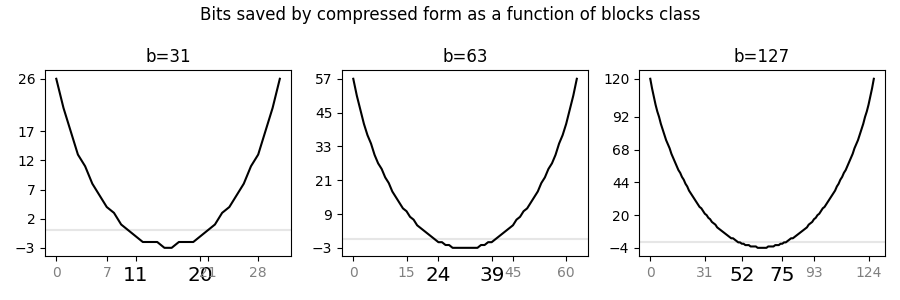
\includegraphics[width=\textwidth]{images/rrr_space_savings}
	}
	\caption[TODO]{Individual graphs present for different block sizes (31, 63, 127), 
    the space saved by using the compressed block representation. We can observe how
    the blocks class influences number of saved bits. Black numbers on the $x$-axis
    denote start and end of the interval where compressed version is even worse
    in space used (negative number of bits saved).
	}
    % can be found on https://github.com/Aj0SK/master-thesis/blob/main/text/images/rrr_space_savings.png
	\label{obr:rrrSpaceSavings}
\end{figure}

For a block size $b$, the random variable $X$ denoting number of ones in a single
block follows a binomial distribution $$X \sim Bin(b, p).$$ As we may observe in
Fig.~\ref{obr:hybridEncodingDistribution}, the probability that block contains
a lot of ones decreases exponentially in a sequence containing only 5\% of ones.
Even in very long sequences, these blocks occur very rarely. This led us to the
idea of an encoding method we call \textit{hybrid encoding}.

\begin{figure}
	\centerline{
		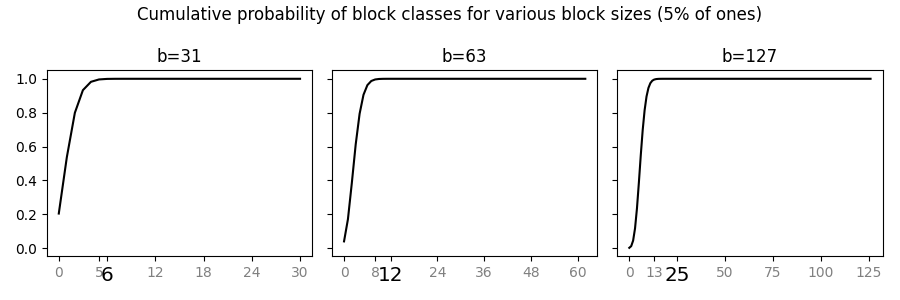
\includegraphics[width=\textwidth]{images/hybrid_encoding_motivation}
	}
	\caption[TODO]{On these 3 graphs, we can see the cumulative distribution
    of blocks classes for the block sizes 31, 63, 127. The frequency of ones is
    fixed to 5\%. Note the marked classes on the $x$-axis. Numbers 6, 12 and
    25 mark the place up to which 99\% of probability distribution lies for
    the block sizes 31, 63 and 127 respectively.
	}
    % Can be found on https://github.com/Aj0SK/master-thesis/blob/main/text/images/hybrid_encoding_motivation.png
	\label{obr:hybridEncodingDistribution}
\end{figure}

The hybrid encoding uses a property that in some sequences blocks with high number
of ones are very rare. Encoding these blocks is not that beneficial as their
compressed representation may take even more bits than the original raw
representation. Storing the whole block may waste space if the number of
ones is big but there are not many possibilities how the block may look.
Although we waste some space by this approach from time to time (for every
block that is densely packed with ones), we can save a small amount of space
by decreasing the number of bits used to store the classes. The main idea
of hybrid encoding is that every block with a class bigger than some threshold
has its class set to this threshold and this means that the block
is stored using full $b$ bits instead of $\lg {b\choose c}$ bits.
Let $c_k$ be a cutoff value. Blocks with class bigger than $c_k$ will not be
encoded but just copied with the class set to $c_k$ no matter what is the
number of ones in them.
\[
    \text{stored class} = 
\begin{cases}
    \#_1(B),& \text{if } \#_1(B) < c_k\\
    c_k,              & \text{otherwise}
\end{cases}
\]
Possible value for blocks class is a number from 0 up to $b$. When the cuttoff $c_k$ is
used, the class of block is a number from 0 up to $c_k$. To possibly save some space on
the bit representation of the blocks class, we need to choose $c_k$ such that
$$\lg (c_k+1) < \lg (b+1).$$ Let us now compare these two representations
and the theoretical space savings that can be obtained.

Let $n$ be a length of the
sequence, $b$ the block size and $C_i$ the number of blocks with class $i$. To simplify the
calculations in this section, we assume that $b+1$ as well as $c_k+1$ is a power of 2 and
$n$ is divisible by $b$.

The first representation takes $$(n/b)\lg (b+1) + \sum_{i=0}^{b} C_i\lg {b\choose i}$$
bits of space with the first and second term being the number of bits that is used by the
classes and offsets respectively. The hybrid representation with cutoff $c_k$ takes
$$(n/b)\lg (c_k+1) + \sum_{i=0}^{c_k-1}C_i\lg {b\choose i} + \sum_{i=c_k}^{b}C_i b$$
bits of space. We would like to find out what is the expected space that we save using the
hybrid encoding. We start by simplifying the expected value of the difference of these
representations:
\begin{align}
E[\Delta\text{space}] &= E\left[(n/b)(\lg(b+1)-\lg(c_k+1)) + \sum_{i=c_k}^{i\leq b}C_i\cdot \left(\lg{b\choose i} - b\right)\right] \nonumber\\
&=(n/b)(\lg(b+1)-\lg(c_k+1)) + \sum_{i=c_k}^{i\leq b}E\left[C_i\cdot \left(\lg{b\choose i} - b\right)\right] \nonumber\\
&=(n/b)(\lg(b+1)-\lg(c_k+1)) + \sum_{i=c_k}^{i\leq b}E\left[C_i\right]\cdot \left(\lg{b\choose i} - b\right) \nonumber\\
E[C_i] &= (n/b)\cdot {b\choose i}\cdot p^i\cdot (1-p)^{b-i} \label{eq:hybrid_encoding_expected_c_i}
\end{align}
Here we mainly used the linearity of the expected value. To compute the expected value of
$C_i$ we used the fact, that number of blocks of a certain class follows binomial
distribution. We know that in the bit sequence, there is $p\%$ of ones. There is $n/b$ blocks
and each has probability ${b\choose i}p^i(1-p)^{b-i}$ to be of class $i$. This probability
is independent from the previous blocks and as we are interested in total number of blocks with
this class, it follows that $C_i$ follows binomial distribution. As
$$C_i \sim Bin\left(n/b, {b\choose i}p^i(1-p)^{b-i}\right)$$ it follows that the expected value
is equal to \ref{eq:hybrid_encoding_expected_c_i}.

We present the expected space saved by hybrid implementation for some chosen values of
$p, b$ and $c_k$ in Fig.~\ref{obr:hybridEncodingTheoretical}.
% TODO: space saved should be used, need to regenerate to 1-x
\begin{figure}
	\centerline{
        \begin{tabular}{l c c c}
            $p$                 & $b$   &   $c_k$   &  {\tt used space}\\
        \hline
            \multirow{7}{*}{5}  &   31  &   7       &   0.83\\
                                &   31  &   15      &   0.91\\
                                &   63  &   15      &   0.91\\
                                &   63  &   31      &   0.95\\
                                &   127 &   7       &   1.86\\
                                &   127 &   15      &   0.93\\
                                &   127 &   63      &   0.98\\
        \end{tabular}
        \hspace{4em}
        \begin{tabular}{l c c c}
            $p$                 & $b$   &   $c_k$   &  {\tt used space}\\
        \hline
            \multirow{7}{*}{10} &   31  &   7       &   0.90\\
                                &   31  &   15      &   0.94\\
                                &   63  &   15      &   0.94\\
                                &   63  &   31      &   0.97\\
                                &   127 &   7       &   2.03\\
                                &   127 &   15      &   1.22\\
                                &   127 &   63      &   0.99\\
        \end{tabular}
        %\hspace{4em}
	}
	\caption[TODO]{
        We may observe the ratio of expected space used by the hybrid implementation to space used by our
        standard RRR implementation for varios percentage of ones in the text -- $p$ as well as for
        different block size -- $b$ and cutoff value -- $c_k$. 
    }
	\label{obr:hybridEncodingTheoretical}
\end{figure}
We may observe, that for some choices of cutoff, we may expect to save roughly 10--17\%
of space compared to the original method. On top of this, hybrid encoding approach has a potential
to be of the same or even better performance as it is easier to decode the blocks
saved in the raw form. However, we should note that hybrid encoding is based on our expectations
that the number of these blocks is low, so the possible speedup may not be very significant.

\paragraph{Balanced sequences}

The previous version of hybrid encoding may work well for sequences with low density of ones.
However, we would also like to use this idea as a viable solution for sequences that contain
similar frequencies of zeroes and ones but still exhibit behaviour that some block classes are
underrepresented. This may, for example, occur when sequence has a property, that it is
globally balanced, but is very unbalanced in some local parts. Then it may be the case, that
blocks with low count of zeroes and ones are more frequent than blocks with balanced counts
of zeroes and ones.

Let us say, that we want to only store $r$ classes instead of all $b+1$ of them. To make
some space saving possible, it must hold that $$\lg r < \lg (b+1).$$
We create a range of classes given by closed interval $[\mathit{cut\_from}, \mathit{cut\_to}]$.
If the blocks class is outside of this range, it is encoded in a standard way. On the other
hand, all the values inside of this interval are mapped to one particular class number and the
corresponding block is stored in a raw form instead of its offset. The special block class value
could be without loss of generality the lowest value $\mathit{cut\_from}$. An example of this
idea can be observed in Fig.~\ref{obr:hybrid_encoding_valley}.
\begin{figure}
	\centerline{
	\begin{tabular}{l|c|c|c|c|c|c|c|c|}
	\cline{2-9}
	\textbf{Class} & 0 & 1 & 2 & 3 & 4 & 5 & 6 & 7          \\ \cline{2-9} 
	\textbf{Hybrid mapping} & 0 & 1 & 2 & 2 & 2 & 2 & 2 & 7 \\ \cline{2-9} 
	\end{tabular}
	}
	\caption[TODO]{Encoding of blocks class. Mapping class values in closed range
    $[\mathit{cut\_from}, \mathit{cut\_to}]$ to single value for $\mathit{cut\_from}=2, \mathit{cut\_to} = 6$}
	\label{obr:hybrid_encoding_valley}
\end{figure}
In this example, the number of different possible class values $r$, is equal to 4.
However, using this representation, we would not save any space as the maximum value
of class is still 7 and we need 3 bits to store it. This would consume the same number
of bits to store as original representation. It is easy to observe, however, that these
values can be mapped into the range $[0, 3]$, thus only consuming two bits per class value.

\begin{figure}
	\centerline{
	\begin{tabular}{l|c|c|c|c|c|c|c|c|}
	\cline{2-9}
	\textbf{Class} & 0 & 1 & 2 & 3 & 4 & 5 & 6 & 7          \\ \cline{2-9} 
	\textbf{Hybrid mapping} & 0 & 1 & 3 & 3 & 3 & 3 & 3 & 2 \\ \cline{2-9} 
	\end{tabular}
	}
	\caption[TODO]{Example of hybrid encoding for balanced sequences.
    $[\mathit{cut\_from}, \mathit{cut\_to}]$ to single value for $\mathit{cut\_from}=2, \mathit{cut\_to} = 6$.
    All possible values can be stored using 2 bits as there are 4 possible values. Hybridly encoded pairs
    have as class value the biggest possible value we can store using 2 bits.}
	\label{obr:hybrid_encoding_valley}
\end{figure}

Space used by this representation is equal to
$$(n/b)\lg (c_k+1) + \sum_{i=0}^{\mathit{cut\_from}-1} C_i\lg {b\choose i}
+ \sum_{i=\mathit{cut\_from}}^{\mathit{cut\_to}}C_i b
+ \sum_{i=\mathit{cut\_to}+1}^{b} C_i\lg {b\choose i}.$$

To summarize, we proposed two ideas how to enhance current implementations of RRR.
First idea is related to the way how blocks are encoded and decoded. We devised a new ordering
that can be nicely combined with divide-and-conquer approach and reuse table decoding subroutine
for smaller sub-problems to which it divides the original problem.

The second idea, targeted on sequences with some special properties, was to just store blocks that
are rare in their original form. By using their original representation, we loose some space on these
rare blocks but save space on every single class value, as we do not need to distinguish between blocks
that have certain classes. We devised two versions of hybrid encoding, one more suitable for bit vectors
that are very sparse and contain small percentage of ones (5--10\%), second, for bit sequences that have
balanced number of zeroes and ones but contain many blocks with either small or big class.